\chapter[Topic]{Topic}

\label{Chap:Topic}

\section{Topic}
Image detection, a critical task in computer vision, involves identifying and locating objects within images. 
Traditional software-based approaches for image detection often face challenges related to processing speed and resource utilization, particularly when dealing with large datasets or real-time applications. In response to these challenges, I propose leveraging Field-Programmable Gate Arrays (FPGAs) to accelerate image detection algorithms in hardware. By offloading computationally intensive tasks to FPGA-based hardware accelerators, we aim to significantly enhance the performance and efficiency of image detection systems.

The integration of FPGA-based hardware acceleration offers several compelling advantages. 
Firstly, FPGAs provide inherent parallelism and customizable hardware architectures, enabling efficient execution of image processing algorithms. 
This parallelism can lead to substantial improvements in processing speed, making real-time image detection feasible for applications such as surveillance, autonomous vehicles, and industrial automation. Additionally, FPGA-based solutions offer flexibility and scalability, allowing for the optimization of hardware resources to suit specific image detection requirements. 
Their adaptability is particularly advantageous in scenarios where the detection algorithms need to be customized or updated frequently.

Furthermore, hardware-accelerated image detection using FPGAs can lead to significant reductions in power consumption compared to traditional CPU-based approaches, making it suitable for resource-constrained environments and embedded systems. 
By harnessing the computational efficiency of FPGA-based acceleration, we can achieve higher throughput and lower latency, thereby improving the responsiveness and effectiveness of image detection systems. 
Overall, this research aims to demonstrate the practical significance and utility of FPGA-based hardware acceleration in advancing the capabilities of image detection technology, paving the way for more efficient and scalable solutions in various domains.

\section{Aims}
This projects aim to:
\begin{itemize}
    \item Demonstrate the feasibility and benefits of FPGA-based hardware acceleration for image detection algorithms.
    \item Demonstrate the control of the image detection algorithm using a RISC-V softcore processor.
    \item Evaluate the performance, efficiency, and scalability of a FPGA-based image detection system.
    \item Investigate the potential applications and use cases of FPGAs for image detection tasks in real-world scenarios.
\end{itemize}

It will not include the development of a new image detection algorithm or method, but rather the implementation of existing algorithm(s) for hardware-acceleration, and the control through a RISC-V softcore processor.

\section{Overview}
The work can be divided into subcomponents to provide a timeline and structure to the project, as dependencies on previous work are required to progress.

\subsection{Hardware}
The work will require the Xilinx Artix 7 XC7A100T FPGA, and a corresponding board to access the FPGA resources and I/O ports.
A Digilent Basys 3 board is available initially for development, however, a Digilent Nexys A7-100T board may be required depending on resource limits.
Both these boards use the Artix 7 XC7A100T FPGA, and have VGA output ports to allow for processed images to be displayed to an external monitor.
A camera module will be connected to the FPGA, and the NEORV32 processor will be used to control the image detection algorithm.
This module has currently not been selected in it's entirety, but initial trials will be conducted with an available VGA OV7670 camera module.
The module has been selected due to it's availability, compatability and previous research \cite{SoCImage} conducted with it.

Figure \ref{fig:overview} below provides an overview of the hardware components and their connections.

\begin{figure}[h]
    \centering
    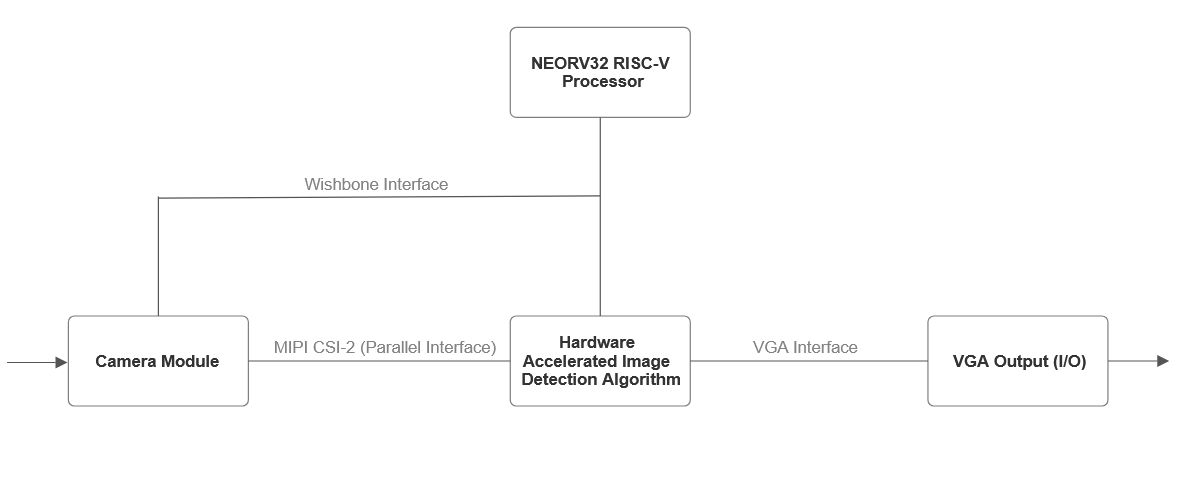
\includegraphics[width=1\textwidth]{Assets/Overview.png}
    \caption{Overview of proposed FPGA-based system.}
    \label{fig:overview}
\end{figure}

\subsection{Softcore Processor}
The NEORV32 RISC-V softcore processor has been selected due to it's highly documented ecosystem, and personal familiarity. 
This processor will be implemented as a SoC on the FPGA, and will be used to control the image detection algorithm and interface with the camera module.
A Wishbone b4 interface will be used to connect the processor to the FPGA.

\subsection{Image Detection Algorithm}
A convolutional neural network has been selected, such as in \cite{Gradient}, to be implemented on the FPGA for image detection.
Existing research has demonstrated that is not as resource intensive as other neural networks, and has noticeable advantages over traditional image detection algorithms.
Furthermore, image analysis is moving in the direction of deep learning algorithms for more complex image detection tasks, such as classification \cite{DCNN}.
By employing a CNN as the algorithm, the project will be able to demonstrate the capabilities of FPGA-based hardware acceleration for deep learning tasks and can be extended to a variety of domains.


\section{Performance Indicators}
The performance indicators of the system to establish the success of the project are provided in Table \ref{tab:performance} below.

\begin{center}
    \small
    \begin{longtable}{lp{0.6\linewidth}}
        \caption{Table of performance indicators.} \label{tab:performance}\\
        \toprule
        Indicator & Description \\
        \midrule
        \endfirsthead
        
        \caption{Performance indicators to assess the success of the project. (continued)} \\
        \toprule
        Indicator & Description \\
        \midrule
        \endhead
        
        \bottomrule
        \multicolumn{2}{r}{\textit{Continued on next page}} \\
        \endfoot
        
        \bottomrule
        \endlastfoot
        
        Algorithm accuracy      & The ability of the system to correctly detect features in an image. \\
        Scalability             & A measure of the limits of the system in terms of image size, image complexity and algorithm complexity \\
        Throughput              & Measured as the number of images processed per time unit \\
        Latency                 & The time delay between acquisition of image and output of results relative to the clock-speed of the Xilinx Artix 7 XC7A100T FPGA \\
        Resource Utilization    & The amount of FPGA resources used to implement the system specified by number of LUTs and BRAM required for implementation \\
    \end{longtable}
\end{center}

\section{Required Resources}
The hardware will be designed using both a Digilent Basys 3 development board for initial prototyping, before ideally being migrated to a Digilent Nexys A7-100T development board, to access more I/O and resources.
This prototyping step is done to demonstrate the implementation on severely resource constrained platforms, as per the scalability performance indicator. 
Both the selected boards have a VGA output, which can be used to display the processed image directly from the FPGA board. 
The specific camera module to be used has not yet been selected, however, a VGA OV7670 camera module which uses an I2C communication protocol is being considered for initial trials.
A VGA monitor will also be required to display the output of the processed image.

Benchmarking materials are dependent on the completed image detection algorithm selected, and cannot be provided at this time. 
Thus, the following resources are required for the project at this stage:

\begin{itemize}
    \item Xilinx Artix 7 XC7A100T FPGA
    \item Digilent Basys 3 FPGA Board
    \item Digilent Nexys A7 100T FPGA Board
    \item Camera Module
    \item VGA OV7670 Camera Module I2C
    \item VGA Monitor
    \item USB Power Supply
    \item VGA to VGA Cable / VGA to HDMI Cable
\end{itemize}
